\documentclass{beamer}
\usepackage[english]{babel}
\usepackage{graphicx, amssymb, amsthm} % Required for inserting images
\usepackage{tikz}
\usetikzlibrary{graphs}

%\usepackage[letterpaper,top=2cm,bottom=2cm,left=3cm,right=3cm,marginparwidth=1.75cm]{geometry}
\usepackage{amsmath}
\usepackage{graphicx}
\usepackage{xcolor}
\usepackage{tikz,xcolor}

\usetikzlibrary{positioning,decorations.pathmorphing,shapes}
\tikzset{main node/.style={circle,draw,minimum size=1cm,inner sep=0pt},}

\definecolor{MUNClaret}{RGB}{134,38,51}

\colorlet{lightgray}{gray!40}

\usecolortheme[named=MUNClaret]{structure}
\usetheme{Warsaw}
\setbeamertemplate{footline}[frame number]

\DeclareMathOperator{\ccr}{c_{cr}}


\title{
  
\includegraphics[width=0.25\textwidth]{../logo/mun_logo.pdf}\\[1em]
  Learning Chaos: Visualizing Sensitivity in the Logistic Map
}
\author{Vasu Manocha \\
MATH 2030 – Memorial University \\
Instructor: Dr. Alexander Bihlo}
\date{Fall 2025}

\begin{document}

\begin{frame}
  \titlepage
\end{frame}

\begin{frame}{Outline}
  \tableofcontents
\end{frame}

\section{Motivation}
\begin{frame}{Why Study Chaos?}
  \begin{block}{Key Ideas}
    \begin{itemize}
      \item Simple deterministic rules can lead to unpredictable, chaotic behavior.
      \item Chaos theory explains real-world phenomena: weather, finance, biology.
      \item The logistic map models population growth, but also period-doubling and chaos.
      \item It's a simple gateway into understanding how complexity emerges from simplicity.
    \end{itemize}
  \end{block}
\end{frame}


\section{The Logistic Map}
\begin{frame}{Model Definition}
  \begin{block}{Logistic Map Formula}
    \[ x_{n+1} = r x_n (1 - x_n) \]
  \end{block}
  \begin{block}{Terms}
    \begin{itemize}
      \item $x_n$: population at step $n$
      \item $r$: growth rate parameter
      \item Behavior depends heavily on $r$
    \end{itemize}
  \end{block}
\end{frame}

\section{Methodology}
\begin{frame}{Computational Methods}
  \begin{block}{Implementation Overview}
    \begin{itemize}
      \item Implemented map in Python with NumPy and Matplotlib
      \item Generated:
        \begin{itemize}
          \item Bifurcation diagrams (full and zoomed)
          \item Sensitivity plots for close initial conditions
          \item Feigenbaum constant estimates
        \end{itemize}
      \item Used Jupyter for reproducible analysis
    \end{itemize}
  \end{block}
\end{frame}
\section{Key Results}
\begin{frame}{Bifurcation Diagram}
  \begin{block}{Diagram}
    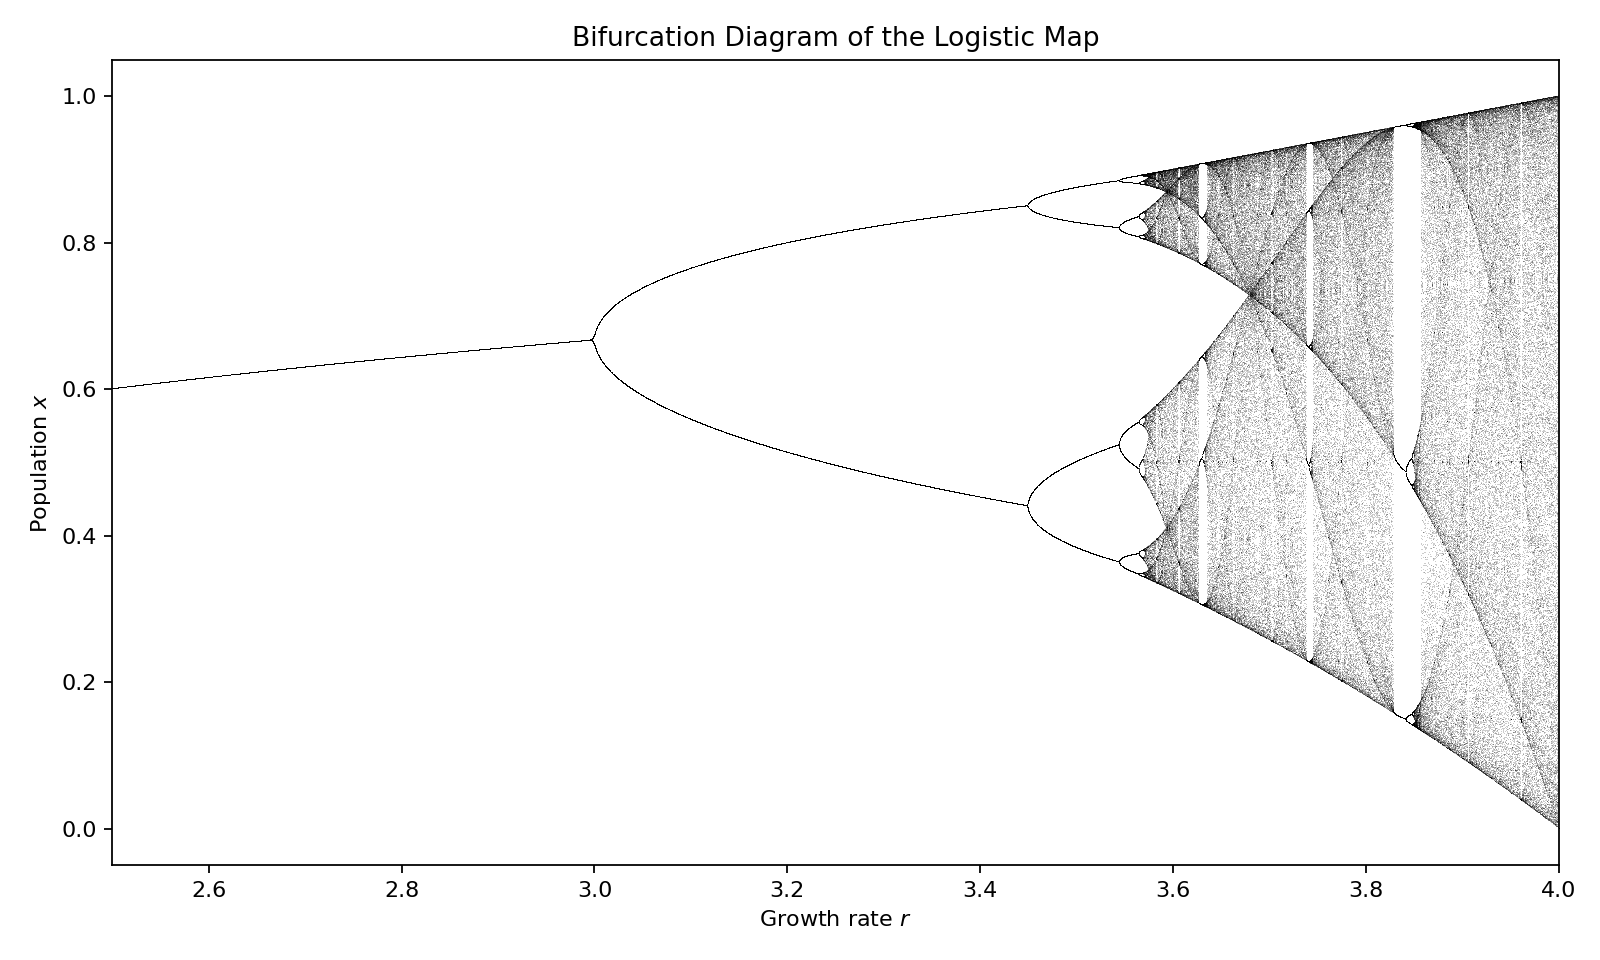
\includegraphics[width=0.9\textwidth]{../Backend/Data/bifurcation_placeholder.png}
  \end{block}
\end{frame}

\begin{frame}{Sensitivity to Initial Conditions}
  \begin{block}{Visualizing Divergence}
    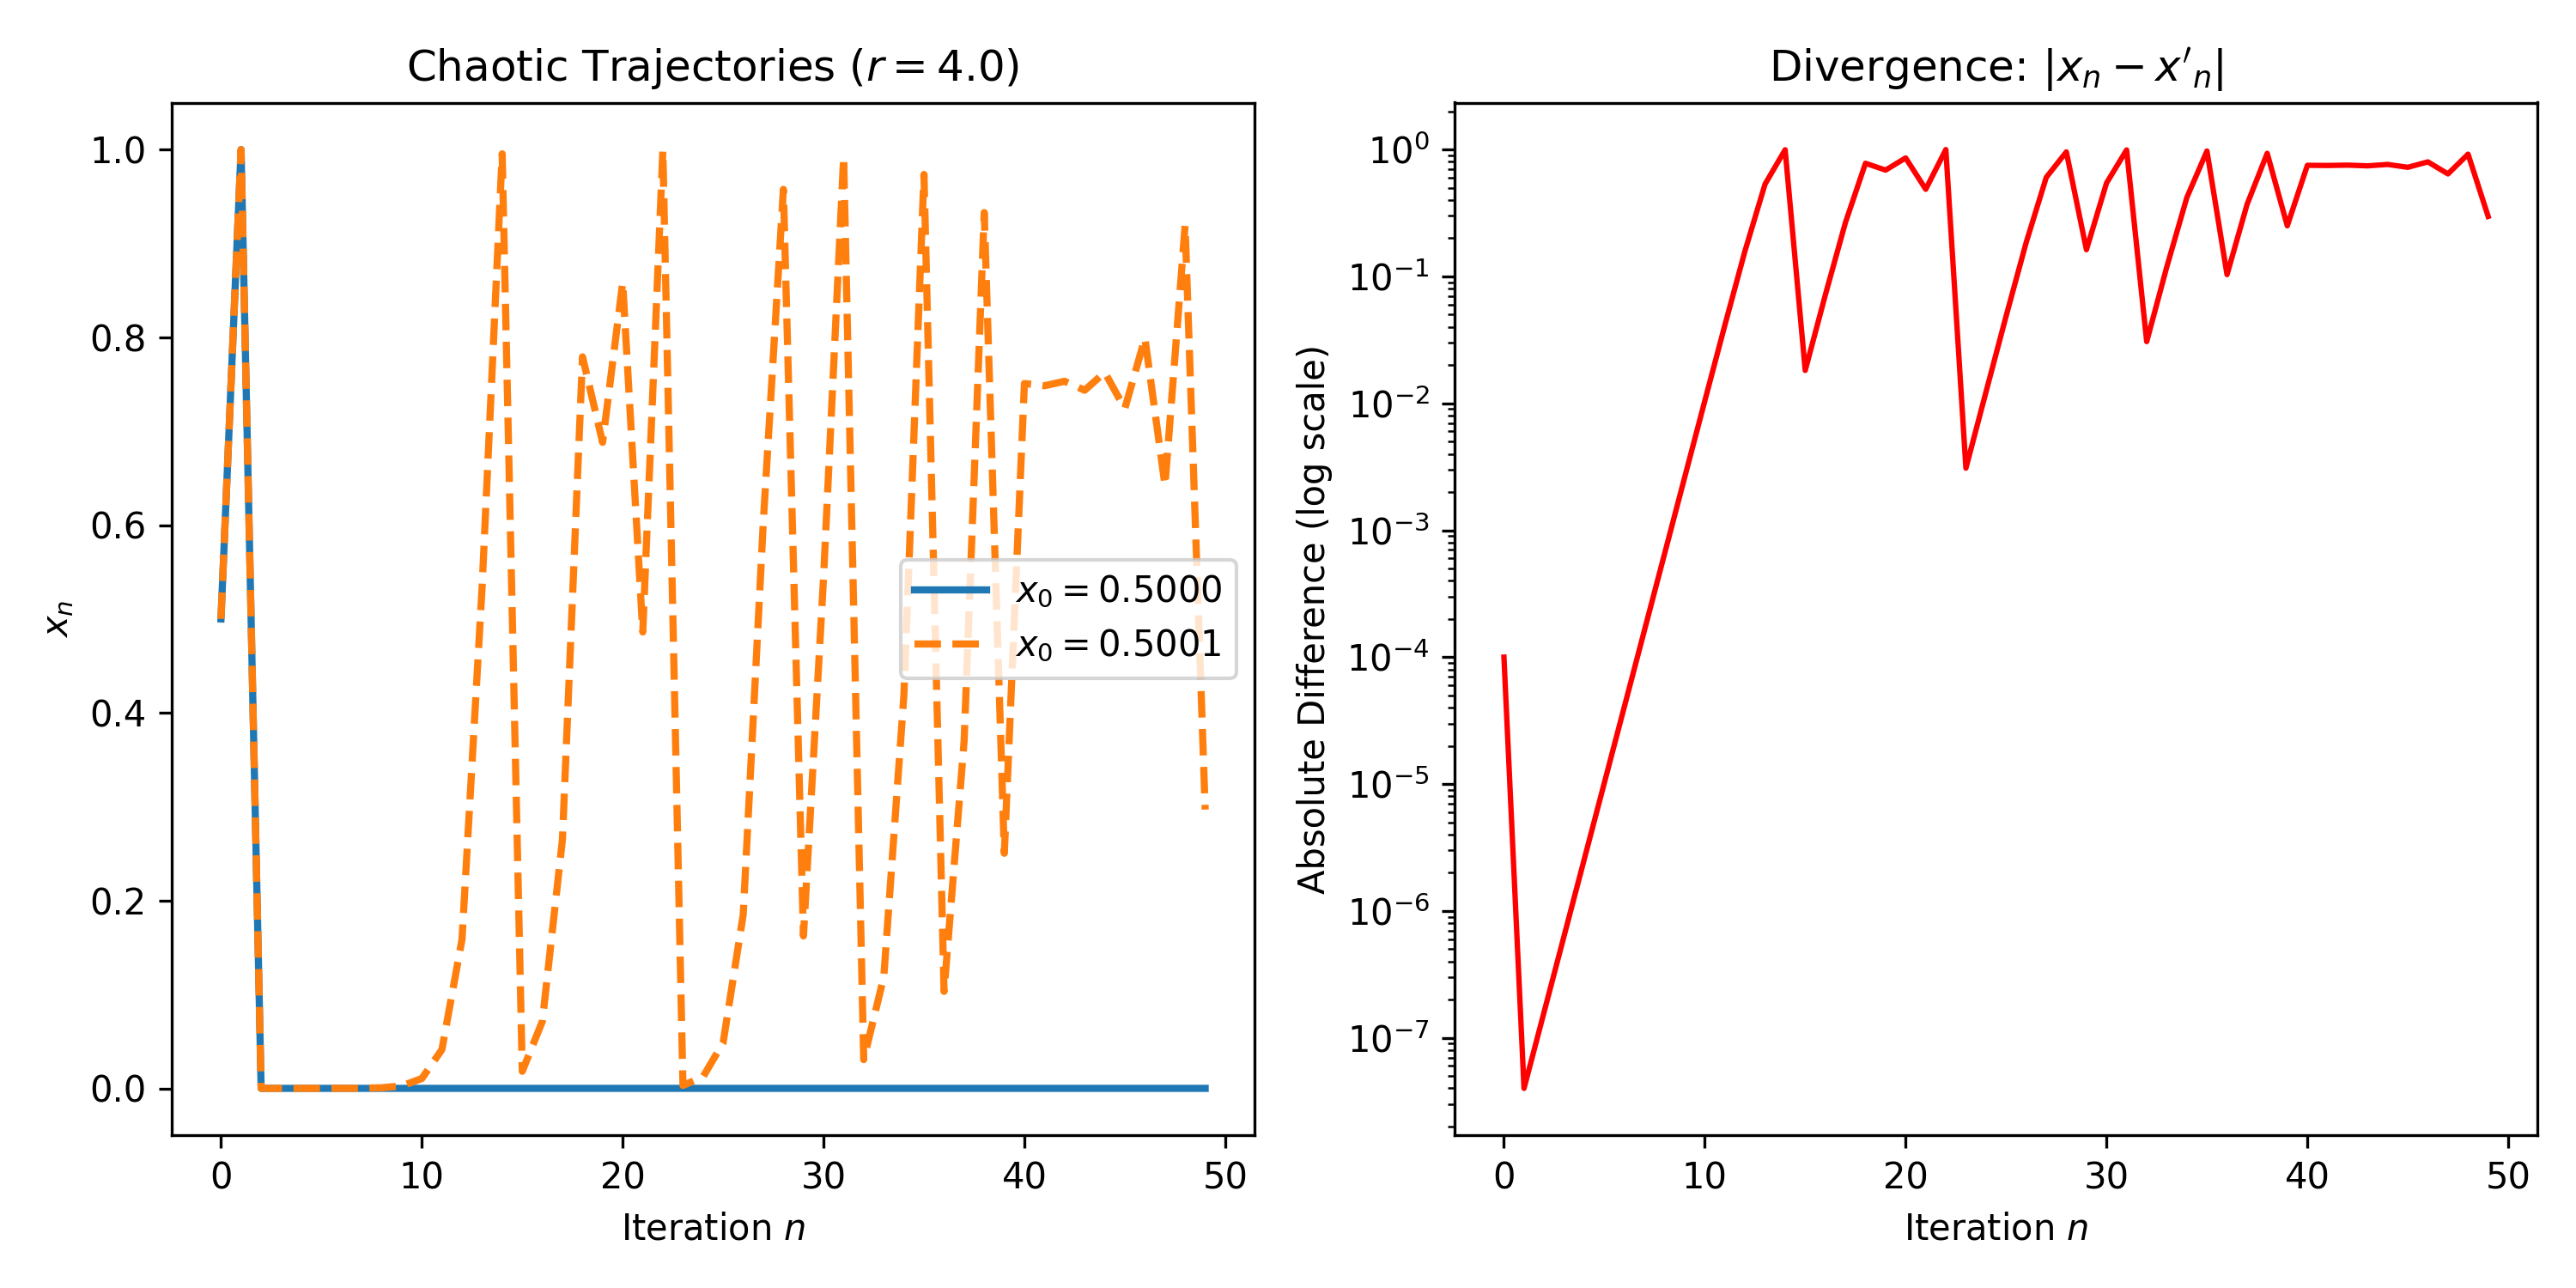
\includegraphics[width=0.9\textwidth]{../Backend/Data/sensitivity_placeholder.png}
  \end{block}
\end{frame}

\begin{frame}{Feigenbaum Constant Estimation}
  \begin{block}{Zoomed Bifurcation with Annotations}
    \centering
    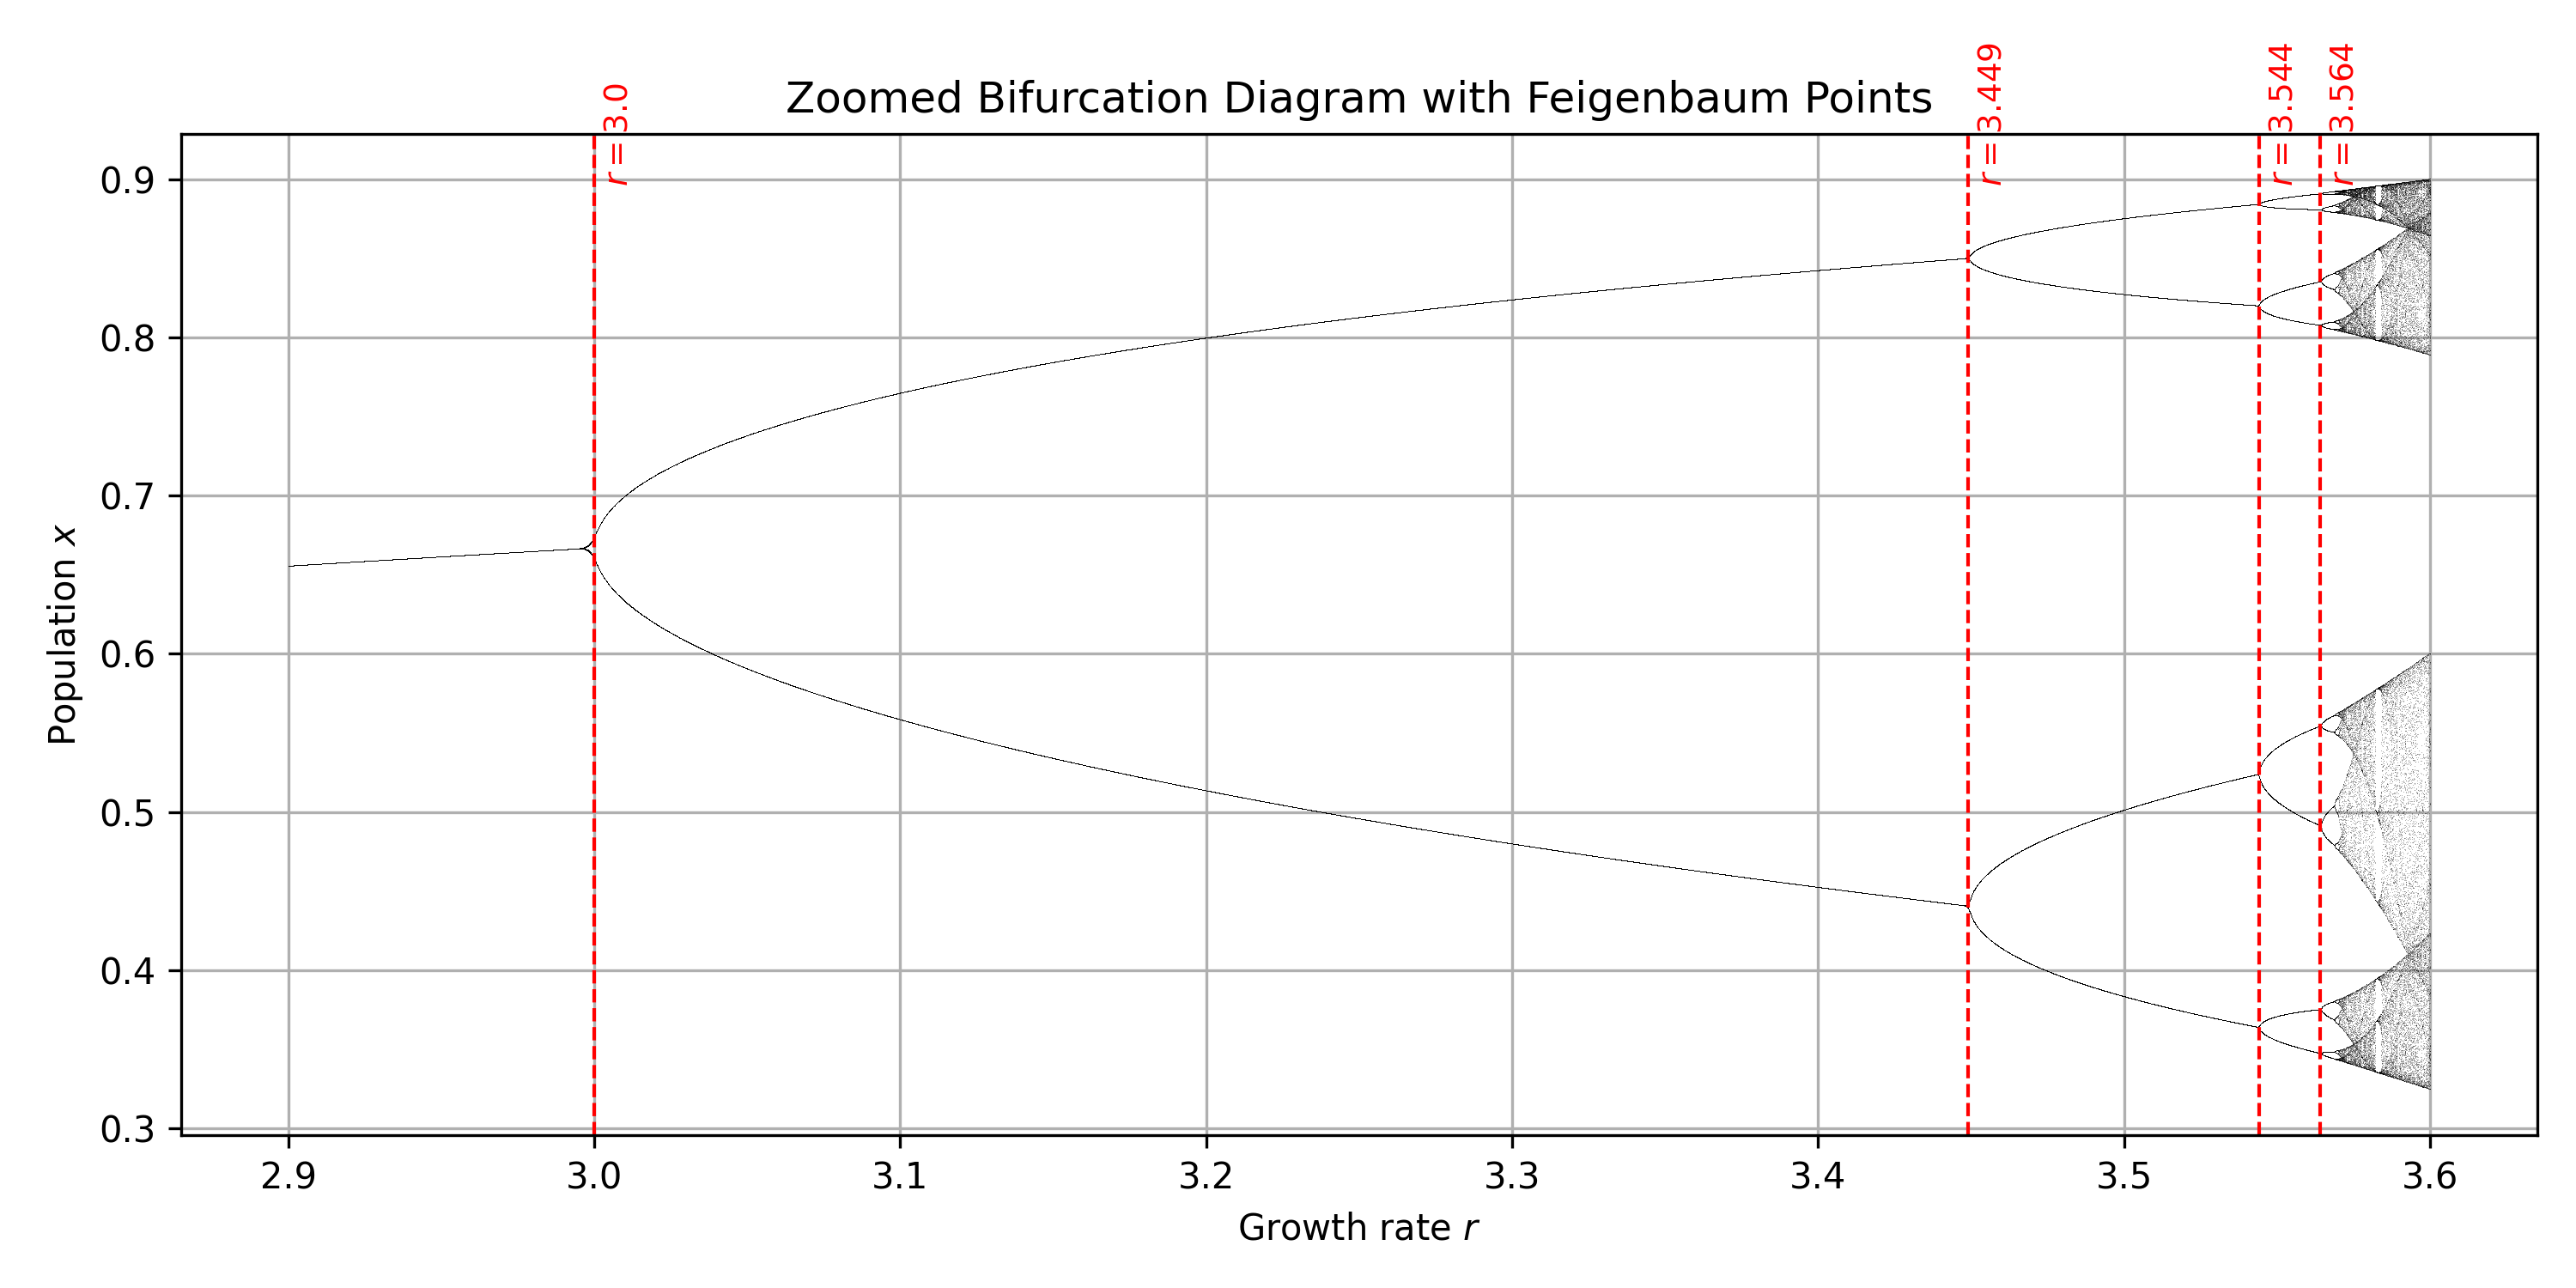
\includegraphics[width=0.78\textwidth]{../Backend/Data/feigenbaum_zoomed_labeled.png}
  \end{block}

  \vspace{-0.5em} % tighten spacing

  \begin{block}{Observation}
    \begin{itemize}
      \item Estimated $\delta_2 \approx 4.7263$, $\delta_3 \approx 4.7500$
      \item Close to theoretical value: $\delta \approx 4.669$
    \end{itemize}
  \end{block}
\end{frame}




\section{Conclusion}
\begin{frame}{Summary}
  \begin{block}{Key Points}
    \begin{itemize}
      \item Visualized how chaos emerges in the logistic map
      \item Demonstrated sensitive dependence and period-doubling
      \item Estimated a universal constant with simple code
    \end{itemize}
  \end{block}
\end{frame}

\begin{frame}{Next Steps}
  \begin{block}{Future Work}
    \begin{itemize}
      \item Automate bifurcation detection
      \item Compute Lyapunov exponents
      \item Explore other chaotic maps (tent, sine)
    \end{itemize}
  \end{block}
\end{frame}

\begin{frame}{Thank You}
  \begin{block}{Questions?}
    \centering
    Thank you for your attention.
  \end{block}
\end{frame}

\end{document}
